\documentclass{article}
\usepackage[utf8]{inputenc}
\usepackage{graphicx}
\usepackage{siunitx}

\title{Physics 111 Lab 02: Acceleration}
\author{Noman Ahmad }
\date{Due Date: March 04, 2021}

\begin{document}

\maketitle

\section{Introduction}
\subsection{Background Information} 
In the previous lab, we looked at objects in motion that had zero-acceleration, also observed as constant velocity. When an object travels with zero-acceleration, it's velocity does not change. In this lab, we observe objects in a non-zero acceleration setting and try to observe how acceleration affect's an object's motion. 
\subsection{Theory and Definitions}
\textbf{Acceleration} is the rate of change of the velocity of an object, just like how velocity was the rate of change of the displacement of an object. In simple terms, acceleration observes how fast an object is speeding up or slowing down. Just like velocity, acceleration has a magnitude and a direction, therefore it is a vector quantity. One of the most common examples of acceleration is acceleration due to gravity as an object free falls. In this case, an object is accelerating downwards at a rate of 9.80\si[per-mode=symbol]{\meter\per\second\squared}. Using the acceleration of an object, we can determine many things about the motion of an object. 
\subsection{Relevant Formula's} 
\textbf{Terms}: initial position \(x_0\), final position \(x\), initial velocity \(v_0\), final velocity \(v\), acceleration \(a\), time \(t\), and acceleration due to gravity \(g\). \\ \\ 
\textbf{Average Acceleration}: \(a=\frac{(v-v_0)}{t}\) \\ \\
\textbf{Final Velocity}: \(v = v_0 + at\) \\ \\ 
\textbf{Final Position}: \(x = x_0 + v_0t + \frac{1}{2}at^2\)

\section{Results} 
\subsection{Setup}
For this lab, we used two different online simulators to observe the effects of acceleration on the motion of an object. In the first simulation, we observed 5 different objects with various accelerations. We were provided the position and velocity graphs and calculated the acceleration of the object, the direction of the acceleration and the total displacement of the object. The second simulation was in regards to an object that underwent acceleration due to gravity. In this simulation, we looked at two scenarios, one where the object is dropped from rest and the other where the object is launched up with an initial velocity. For this simulation, we observed how the position and the velocity of an object can change when the acceleration acting on the object is due to gravity. 
\subsection{Constant Accelerated Motion} 
In order to complete the motion table, we had to determine the initial and final velocities of the object based on the graph's, and then use the formula's to calculate the acceleration and the total displacement. In order to determine the direction of acceleration, we observe the motion of the object and use some intuition. For example, if the object is free falling, then its acceleration must be in the -y direction. 

\subsubsection{Sample Calculation} 
The following is a sample calculation for motion 3: \\ \\
\textbf{Observed Values}: \(v_0 = 0\si[per-mode=symbol]{\meter\per\second}\), \(v = 10.0\si[per-mode=symbol]{\meter\per\second}\), \(x_0 = 0\si[per-mode=symbol]{\meter}\), \(x=50.0\si[per-mode=symbol]{\meter}\), \(t=10s\). \\ \\ 
\textbf{Acceleration}: \(a = \frac{(v-v_0)}{t}\) \Rightarrow \(a = \frac{10\si[per-mode=symbol]{\meter\per\second}}{10s}\) \Rightarrow {\(a = 1.0\si[per-mode=symbol]{\meter\per\second\squared}\)}. \\ \\ 
\textbf{Displacement} : \(x = x_0 + v_0t + \frac{1}{2}at^2\) \Rightarrow \(x = \frac{1}{2}(1.0)(10)^2\) \Rightarrow \(x = 50\si[per-mode=symbol]{\meter}\). \\ \\ 
If we notice, our calculated displacement using the formula is the same as the displacement observed in the position graph, so our calculations are correct. 

\subsubsection{Motion Table}
The following table is the result of the motion calculations of all 5 objects. 
\begin{center} 
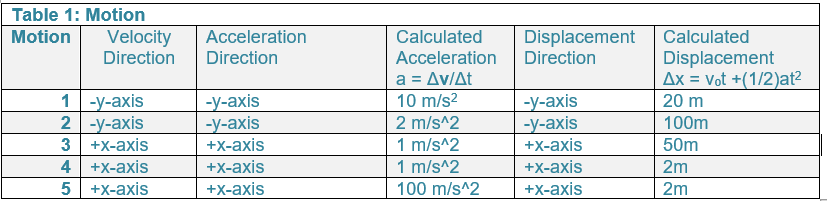
\includegraphics[scale=0.5]{motion_table1.png}
\end{center}

\subsubsection{Observations} 
The interesting observation here is that the directions of displacement, velocity, and acceleration are the same for all five cases. While this might hold true in these cases, this does not always have to be true. For example, when you press brake on a car, the acceleration is negative which would be causing the velocity to decrease to rest, however at the same time the velocity is still positive until it finally reaches rest. This shows that the directions of displacement, velocity, and acceleration vectors do not always have to be the same. 

\subsection{Acceleration Due To Gravity} 
When an object is dropped or launched in the air, the acceleration acting on the object is \(g = 9.8\si[per-mode=symbol]{\meter\per\second\squared}\). This acceleration is due to gravity, causing the object to always reach the ground, whether it was dropped or launched into the air. In this part of the lab, we examine objects as they are dropped and launched into the air.
\subsubsection{Falling From Rest}
In this problem, we are examining a ball that is falling from rest under the influence of gravity (neglecting air resistance), and we want to determine how long it will take for the ball to drop 20m, from rest. [Problem 19] \\ \\  
\textbf{Givens}: \(v_0 = 0\si[per-mode=symbol]{\meter\per\second}\) , \(x_0 = 0\si[per-mode=symbol]{\meter}\), \(x = -20\si[per-mode=symbol]{\meter}\), \(a = g = 9.8\si[per-mode=symbol]{\meter\per\second\squared}\) \\ \\ 
\textbf{Time}: \(x = x_0 + v_0t + \frac{1}{2}at^2\) \Rightarrow \(x = +\frac{1}{2}gt^2\) \Rightarrow \(t = \sqrt{\frac{2x}{g}}\) \Rightarrow \(t=\sqrt{\frac{40}{9.8}}\) \Rightarrow \(t = 2.02s\) 

\subsubsection{Launching Objects Into The Air}
For this problem, we observe a ball that is being launched in the air at 20m/s from the ground, and we want to calculate how long it takes for the ball to return back to the ground, under the influence of gravity (neglecting air resistance). We also want to calculate how high the ball reaches (maximum height). [Problem 28 \& 29] \\ \\ 
\textbf{Initial Observations:} We know that when the ball is thrown upwards, it will decelerate until it reaches it's maximum height where the velocity will be at rest momentarily, then accelerate downwards again, the time it takes for the ball to reach it's peak will be equivalent to the time it takes to reach the ground again. Therefore, we only need to calculate once, and double the value. \\ \\ 
\textbf{First Half Of Motion: } \(v_0 = 20\si[per-mode=symbol]{\meter\per\second}\), \(v = 0\si[per-mode=symbol]{\meter\per\second}\),  \(a=-g=-9.8\si[per-mode=symbol]{\meter\per\second\squared}\). \\\\
\textbf{Total Time:} \(v = v_0 + at\) \Rightarrow \(t_{half} = \frac{(v-v_0)}{-g}\) \Rightarrow \(t_{full} = \frac{2(v-v_0)}{-g}\) \Rightarrow \(t_{full} = \frac{-40}{-9.8}\) \Rightarrow \(t_{full} = 4.08s\) and \(t_{half} = 2.04s\) \\ \\ 
\textbf{Maximum Height: } \(x = x_0 + v_0t + \frac{1}{2}gt^2\) \Rightarrow \(x = 20(2.04) + \frac{1}{2}(-9.8)(2.04)^2\) \Rightarrow \(x = 20.41m\). \\ \\ 
For finding the maximum height, I use the time it takes to reach the top as if it were launched from the ground with the 20m/s initial velocity. I could have chosen to do this by looking at how far it drops in the second half of the motion, and the answer would still be the same. 
\subsubsection{Percent Error Calculations} 
The problems that we just solved using the formulas have been demonstrated in the second online simulator as mentioned earlier. The object in the graphs provided follows the same motion. Now, we have to calculate the percentage error between our calculated time and height to the one given by the graphs. [Problem 34 \& 35] \\ \\ 
\textbf{Calculated \& Observed Values}: \(t_{calc} = 4.08s\), \(t_{obs} = 4s\), \(x_{calc} = 20.41m\), \(x_{obs} = 20m\). \\\\
\textbf{Time Percentage Error:} \(100 \cdot \frac{|t_{calc} - t_{obs}|}{t_{calc}}\) \Rightarrow \(100 \cdot \frac{|4.08-4|}{4.08}\) \Rightarrow \(Error= 1.96\%\) \\\\
\textbf{Height Percentage Error:} \(100 \cdot \frac{|x_{calc} - x_{obs}|}{x_{calc}}\) \Rightarrow \(100 \cdot \frac{|20.41-20|}{20.41}\) \Rightarrow \(Error= 2\%\) 

\subsubsection{Average Speed Vs. Average Velocity}
In the next few problems, we observed the differences in average speed and average velocity when launched and when dropped. [Problem 37 \& 38] \\ \\ 
\textbf{Average Speed When Dropped: } \(S_{avg} = \frac{distance}{time}\) \Rightarrow \frac{20m}{2s} \Rightarrow 10\si[per-mode=symbol]{\meter\per\second}. \\ \\
\textbf{Average Velocity When Dropped: } \(V_{avg} = \frac{displacement}{time}\) \Rightarrow \frac{-20m}{2s} \Rightarrow -10\si[per-mode=symbol]{\meter\per\second}. \\ \\
\textbf{Average Speed When Launched: } \(S_{avg} = \frac{distance}{time}\) \Rightarrow \frac{40m}{4s} \Rightarrow 10\si[per-mode=symbol]{\meter\per\second}. \\ \\
\textbf{Average Velocity When Launched: } \(V_{avg} = \frac{displacement}{time}\) \Rightarrow \frac{0m}{4s} \Rightarrow 0\si[per-mode=symbol]{\meter\per\second}

\section{Post-Lab Questions}
\subsection{Problem 1}
For this problem, We had to complete the ranking exercise and add a screenshot of our completed exercise. [Problem 40]
\begin{center} 
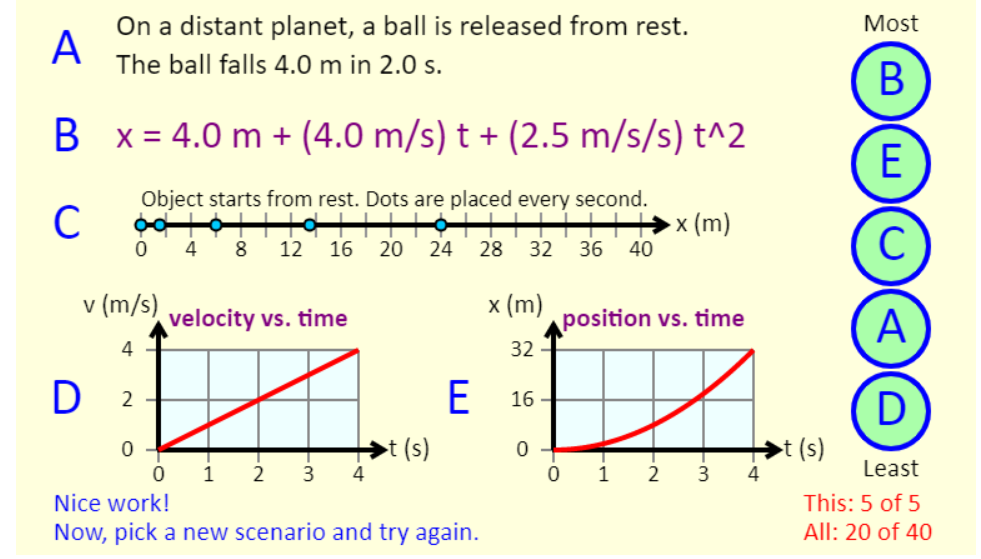
\includegraphics[scale=0.5]{ranking_acceleration.PNG}
\end{center}
\subsection{Problem 2} 
The position \(x(t)\) of a particle as a function of time \(t\) is given by the equation \(x(t) = (3m/s)t - (5m/s^2)t^2\). What is the average velocity of the particle between t = 0.30 s and t = 0.40s? [Problem 41] \\ \\ 
\textbf{Average Velocity}: \(v_{avg} = \frac{(x-x_0)}{t}\) \Rightarrow \frac{((3(0.4) - 5(0.4)^2))-((3(0.3) -5(0.3)^2))}{0.1} \Rightarrow -0.5\si[per-mode=symbol]{\meter\per\second}.
\subsection{Problem 3} 
A captain orders his starship to accelerate from rest at a rate of g. How many days does it take the starship to reach 10\% of the speed of light? [Problem 42] \\ \\ 
\textbf{Time Needed}: \(v = v_0 + at\) \Rightarrow \(t = \frac{(v-v_0)}{a}\) \Rightarrow \(t = \frac{v_{light}}{10g}\) \Rightarrow \frac{3.0\cdot10^8}{10 \cdot 9.80} \Rightarrow 306141224.49 \Rightarrow \(3.06 \cdot 10^6s\). \\ \\
\textbf{Days Needed}: 1 day = 86400s \Rightarrow \(t = 86400(3.06\cdot10^6)\) \Rightarrow \(2.64\cdot10^{11}\) days. 

\subsection{Problem 4} 
The figure shows a graph of the velocity of an object as a function of time. What is the acceleration of the object at the following times? [Problem 43]
\begin{center} 
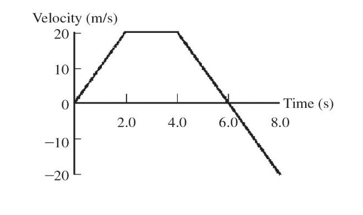
\includegraphics[scale=0.6]{problem43.PNG}
\end{center}
\subsubsection{Instantaneous Acceleration at 1.0s}  
This is just the slope of the initial line that starts at t=0s, and ends at t=2s. The slope here is 10, therefore the acceleration is 10\si[per-mode=symbol]{\meter\per\second\squared}. 
\subsubsection{Instantaneous Acceleration at 3.0s}
Here the velocity is constant, therefore the acceleration is 0\si[per-mode=symbol]{\meter\per\second\squared}. 
\subsubsection{Instantaneous Acceleration at 5.0s} Here we would take the slope of the line segment that begins at t=4.0s and ends at t=8.0s. The slope of that line is -10, therefore the acceleration at this point will also be -10\si[per-mode=symbol]{\meter\per\second\squared}.
\subsection{Problem 5}
The graph in the figure shows the velocity of a particle as it travels along the x-axis. [Problem 44] 
\begin{center} 
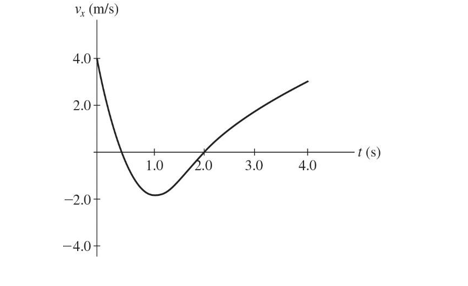
\includegraphics[scale=0.5]{problem44.PNG}
\end{center} 
\subsubsection{Direction of Acceleration at 0.5s} At this time, the velocity of the object is 0m/s, meaning it is at rest, however immediately afterwards, the objects continues to slow down. Therefore, the acceleration is negative causing the object to decelerate and lose speed. The direction of the acceleration is in the -x. 
\subsubsection{Direction of Acceleration at 3.0s} Similar to previous reasoning, the magnitude of the velocity of the object is increasing, therefore there is positive acceleration causing it to get faster, therefore the acceleration's direction is +x. 
\subsubsection{Average Acceleration} \(a_{avg} = \frac{(v-v_0)}{t}\) \Rightarrow \frac{(v(4)-v(2))}{4-2} \Rightarrow \frac{3}{2}\si[per-mode=symbol]{\meter\per\second\squared}  
\subsubsection{Instantaneous Acceleration} The instantaneous acceleration is when the velocity curve changes it's direction, therefore the acceleration was decreasing then reached 0 momentarily, and then started increasing again. The point on the curve where this is true is at t=1.0s. 
\section{Discussion} 
In this lab, we used a simulation to get a better understanding of the way acceleration affects the motion of an object. Our experiment was successful because of the low percentage errors that we received (<2\%). I believe this minimal error was due to the simulation having rounded the acceleration due to gravity up to 10\si[per-mode=symbol]{\meter\per\second\squared} (i think), and therefore not exactly accurate entirely. We were also able to understand how acceleration due to gravity affects an object whether it is launched or dropped. The time it takes to reach the maximum height will be equal to the time it takes to drop down from maximum height. I also noticed that the way we look at acceleration in comparison to velocity is the same way we look at velocity in comparison to position. Looking for average and instantaneous acceleration on a velocity curve works the same way as looking for average and instantaneous velocity on a position curve, and i think this makes a lot of intuitive sense. The most important thing however, was that the direction of the acceleration is not always the same as the direction of the velocity. The best example of this is when a launched up with a positive velocity, and the acceleration due to gravity is slowing it down with a negative acceleration. In conclusion, I was able to get a better understanding of constant acceleration motion in today's lab and was able to conduct a successful experiment on it. 


\end{document}

